This chapter presents background information on virtualization and confinement
technologies in Linux and other Unix-like operating systems. It also presents a detailed
history and examination of eBPF and discusses its applications in the domains of computer
security, performance monitoring, and beyond.

\section{Virtualization Technologies}%
\label{s:virtualization-bg}

\subsection{Namespaces}%
\label{ss:namespaces-bg}

\subsection{Process Control Groups}%
\label{ss:cgroups-bg}

\subsection{Hypervisors and Virtual Machines}%
\label{ss:vms-bg}




\section{Confinement Technologies}%
\label{s:confinement-bg}

\subsection{FreeBSD Jails}%
\label{ss:jails-bg}

\subsection{OpenBSD Pledge and Unveil}%
\label{ss:pledge-bg}

\subsection{Linux Seccomp and Seccomp-BPF}%
\label{ss:seccomp-bg}

\subsection{Unix DAC}%
\label{ss:unix-dac-bg}

\subsection{Linux MAC}%
\label{ss:linux-mac-bg}




\section{Linux Containers}%
\label{s:containers-bg}




\section{Extended BPF}%
\label{s:ebpf-bg}

eBPF stands for \enquote{Extended Berkeley Packet Filter}, though in reality it has very
little to do with Berkeley, packets, or filtering in its current form.  In a nutshell,
eBPF is a Linux kernel technology that supports dynamic monitoring of a production system
through the attachment of special \enquote{hooks} called BPF programs to specific kernel
interfaces and userspace functions. In this section, we discuss the origins of eBPF, its
components and how they work, its applications under the Linux kernel, and how it has
evolved over time.

\subsection{Origins of BPF\@: An Efficient Packet Filtering System}%
\label{ss:origins-of-bpf-bg}

The original Berkeley Packet Filter, hereafter referred to as classic BPF or cBPF, arose
out of a need to implement a more efficient packet filtering mechanism for BSD Unix.
McCanne and Jacobson~\cite{mccanne1993_bpf} published their work on cBPF in 1993, marking
an improvement over existing mechanisms in a number of ways. Many of the reasons why
classic BPF was such an improvement over the status quo are still relevant when discussing
\textit{eBPF}, and so we will briefly cover them here as well.

In essence, classic BPF was a \textit{register virtual machine} designed to take packets
as input and produce \textit{filtering decisions} as output. These filtering decisions
could then used to make decisions about whether a packet should be passed down to a more
complex pipeline for further analysis. The key insight behind classic BPF was that these
filtering decisions could be made more efficiently in \textit{kernelspace}, the part of
the operating system that runs in protection ring 0\footnote{In practice, ring 0 is the
highest real level of memory protection offered by the CPU (although negative rings do
exist on modern CPUs, they are, in fact, merely partitions of ring 0)~\todo{CITE}. Code
that runs in ring 0 is said to run with \textit{supervisor privileges}.} and which is most
commonly associated with any parts of the operating system that do not run in
\textit{userland} (i.e.~the context of an ordinary user process). This provides
a considerable performance advantage over conventional approaches to network monitoring.
A typical network monitor runs in \textit{userspace}, meaning that packets need to be
copied over from kernelspace before they can be properly analyzed. This is an expensive
operation, requiring several context switches and potentially sleeping in the event of
a page fault~\cite{mccanne1993_bpf}. By applying filtering logic in the kernel, this
expensive copying could be skipped for packets that would be discarded or ignored by the
network monitor anyway.

\begin{figure}[htbp]
  \centering
  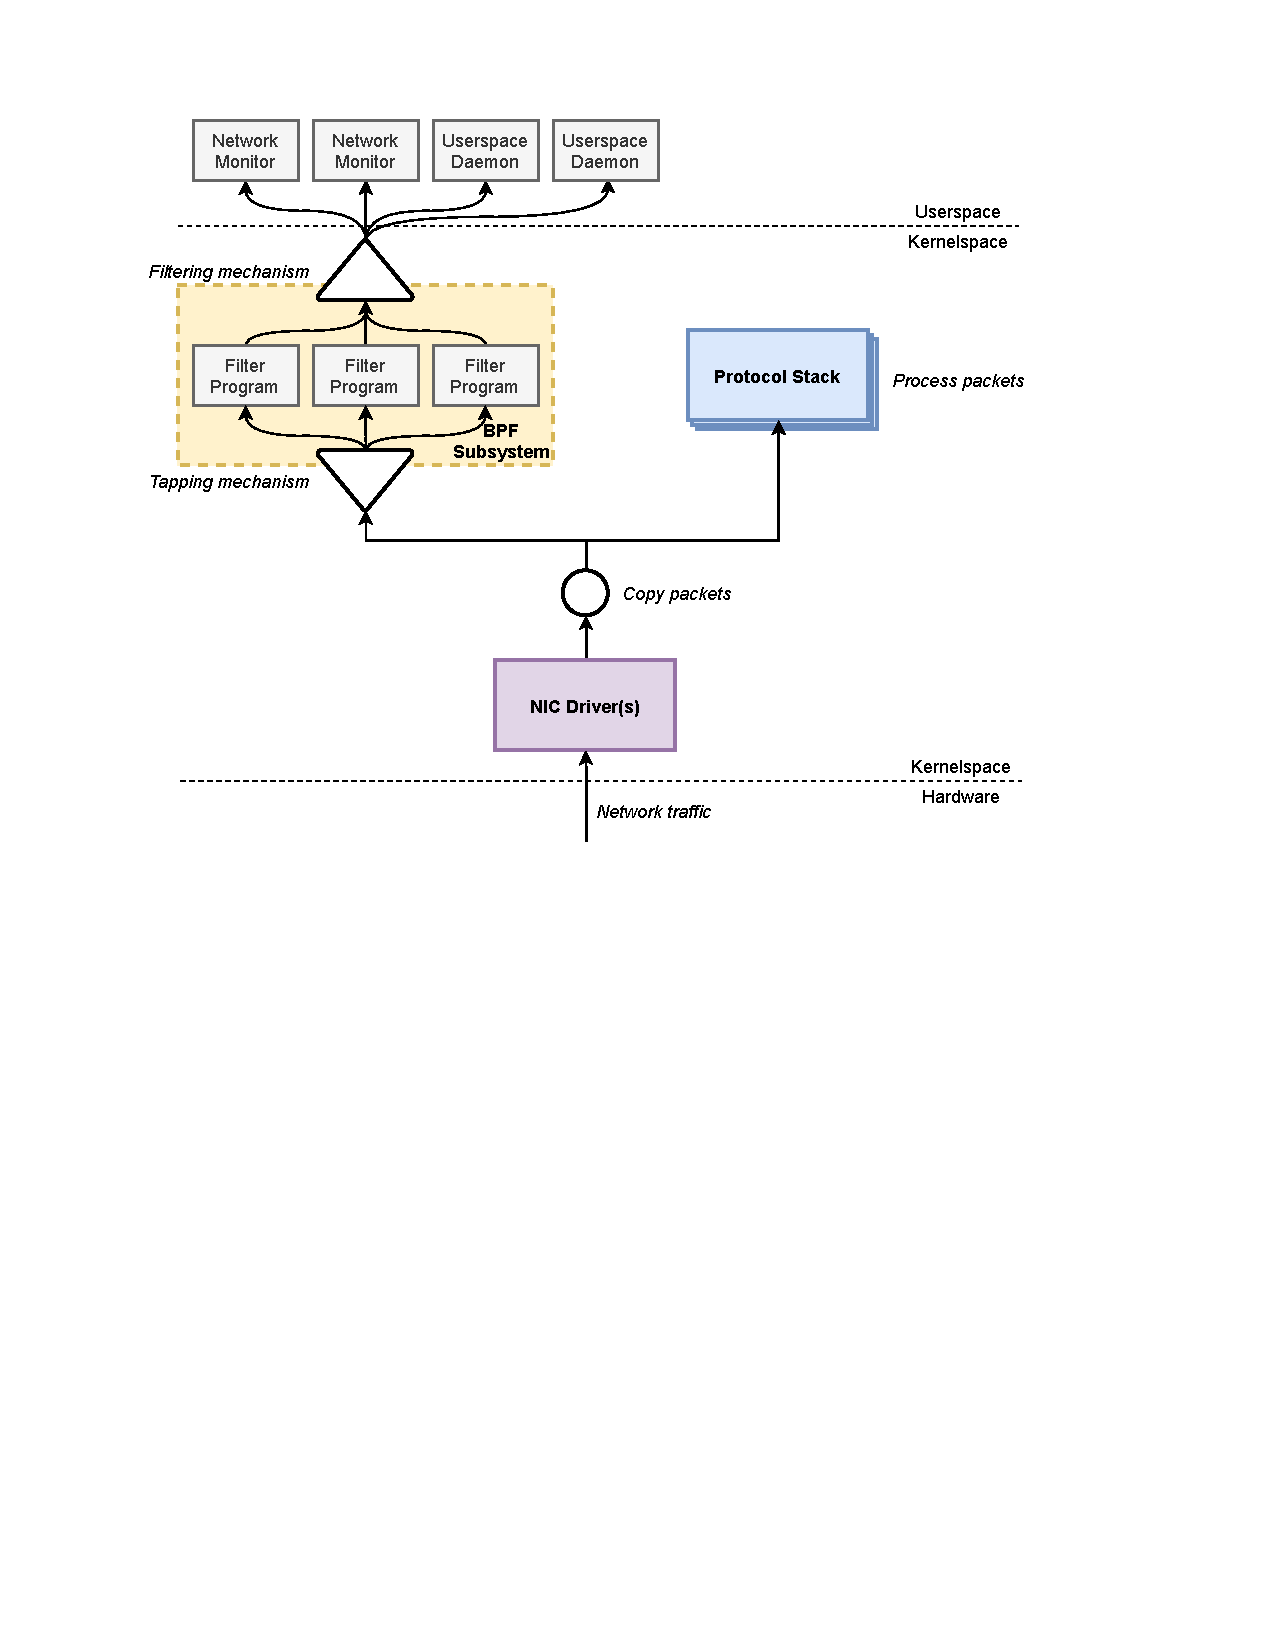
\includegraphics[width=0.8\linewidth]{figs/background/classic-bpf.pdf}
  \caption{The classic BPF architecture. Adapted from McCanne and Jacobson~\cite{mccanne1993_bpf}.}%
  \label{fig:classic-bpf}
\end{figure}

\subsection{eBPF Programs}%
\label{ss:bpf-programs-bg}

\subsection{eBPF Maps}%
\label{ss:bpf-maps-bg}

\subsection{The Verifier}%
\label{ss:verifier-bg}

\subsection{eBPF Use Cases}%
\label{ss:ebpf-use-cases-bg}

\subsection{How eBPF Has Evolved Over Time}%
\label{ss:ebpf-evolution-bg}

